\documentclass{standalone}
\usepackage{tikz}
\usetikzlibrary{patterns, positioning}
\usepackage[sfdefault]{ClearSans} %% option 'sfdefault' activates Clear Sans as the default text font
\usepackage[T1]{fontenc}

\begin{document}
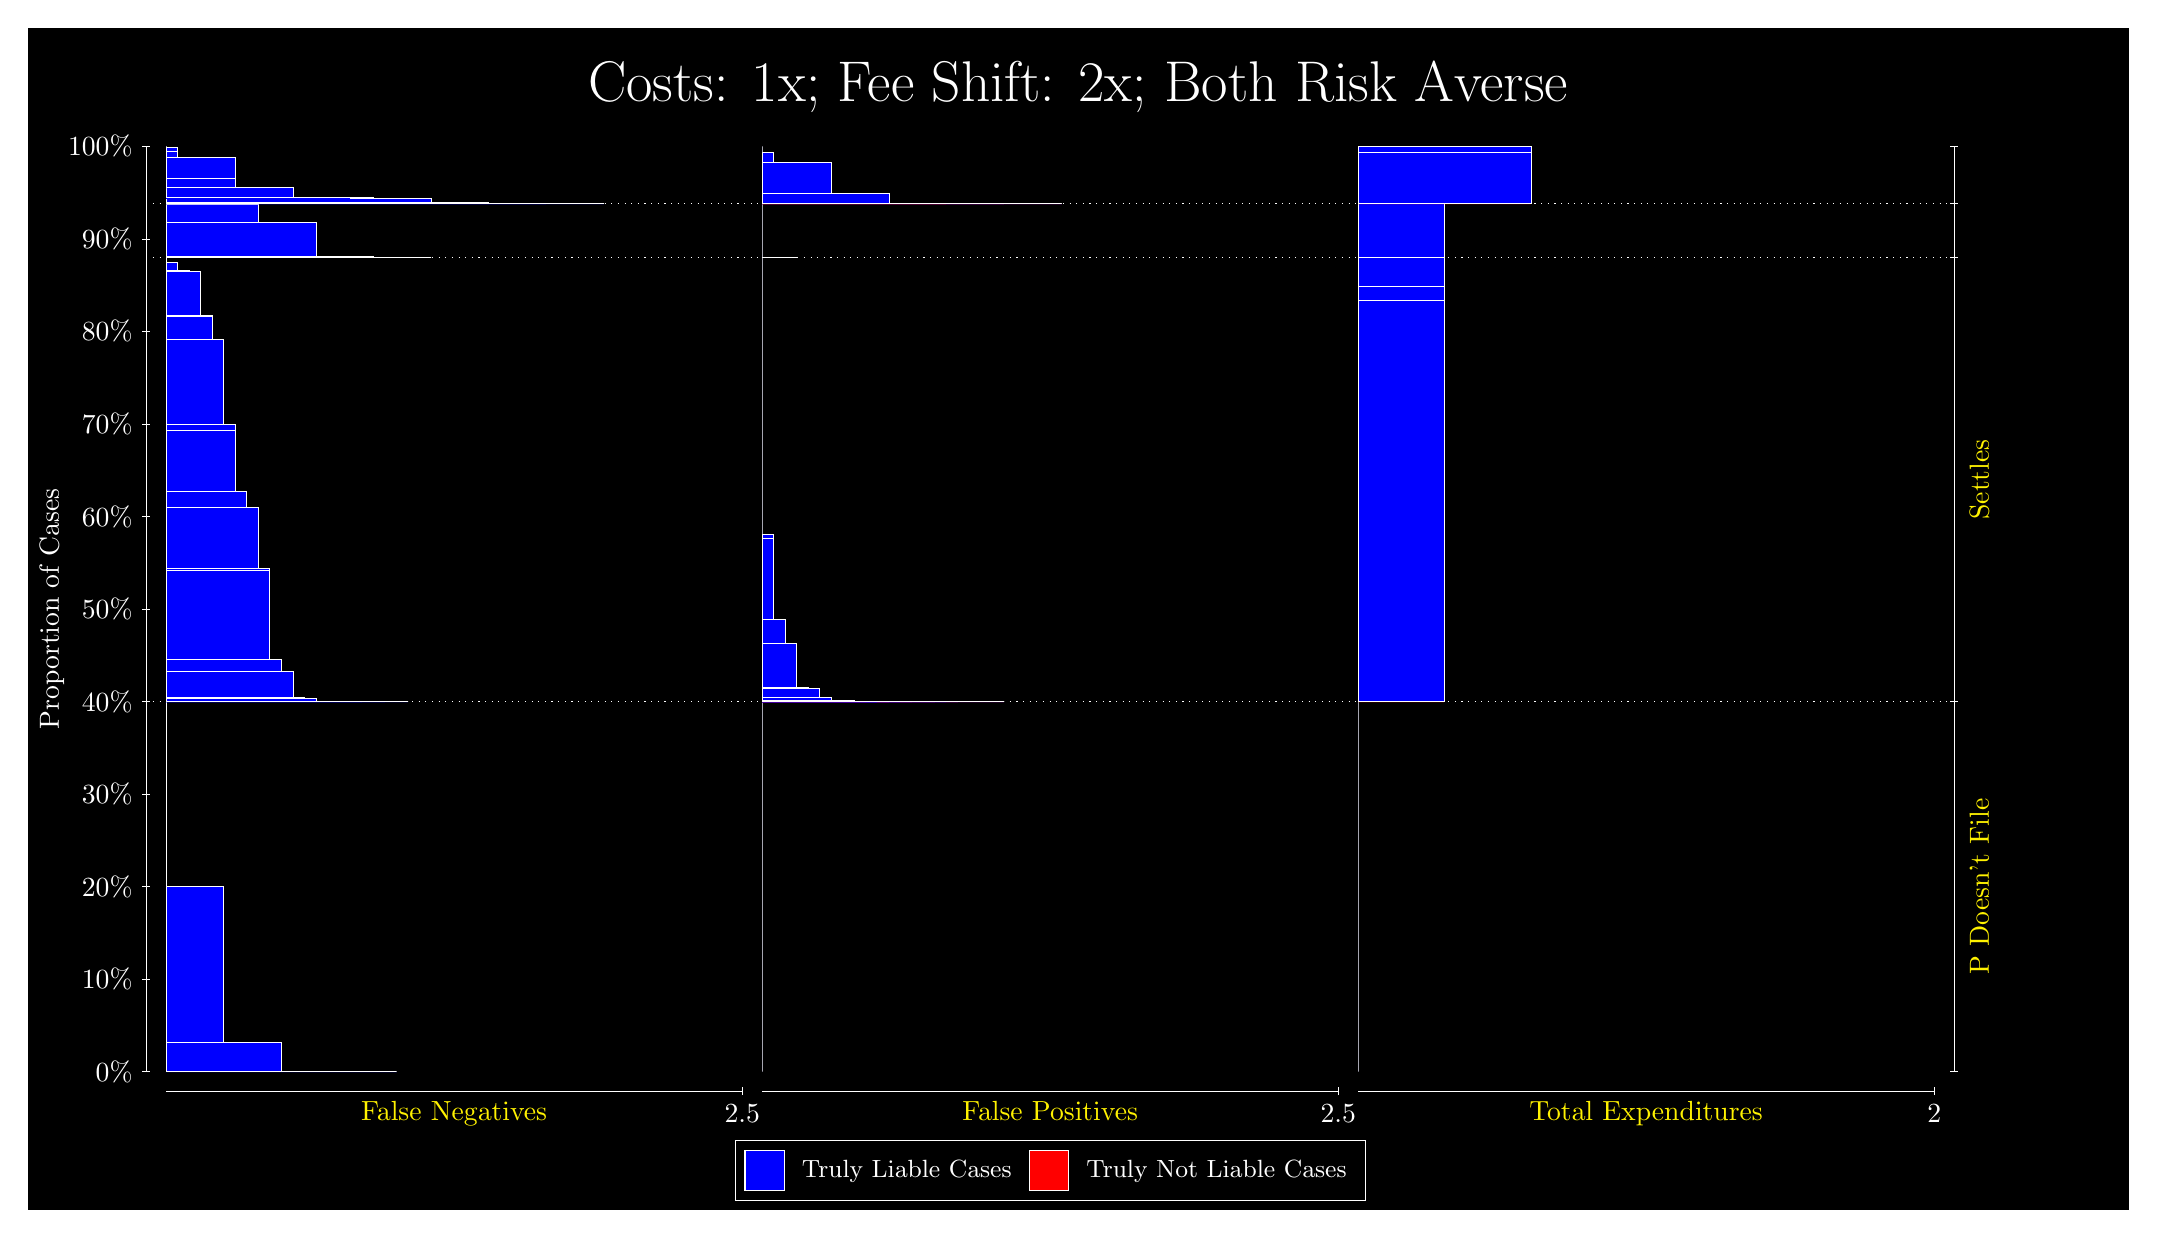
\begin{tikzpicture}
\draw[fill=black] (0,0) rectangle (26.667,15);
\draw[text=white] (0,13.5) rectangle (26.667,15) node[midway] {\huge Costs: 1x; Fee Shift: 2x; Both Risk Averse};
\draw[white, very thin] (1.5,1.75) -- (1.5,13.5);
\node[rotate=90, text=white, anchor=center] at (0.3, 7.625) {Proportion of Cases};
\draw[white, very thin] (1.45,1.75) -- (1.55,1.75);
\node[text=white, anchor=east] at (1.45, 1.75) {0\%};
\draw[white, very thin] (1.45,2.925) -- (1.55,2.925);
\node[text=white, anchor=east] at (1.45, 2.925) {10\%};
\draw[white, very thin] (1.45,4.1) -- (1.55,4.1);
\node[text=white, anchor=east] at (1.45, 4.1) {20\%};
\draw[white, very thin] (1.45,5.275) -- (1.55,5.275);
\node[text=white, anchor=east] at (1.45, 5.275) {30\%};
\draw[white, very thin] (1.45,6.45) -- (1.55,6.45);
\node[text=white, anchor=east] at (1.45, 6.45) {40\%};
\draw[white, very thin] (1.45,7.625) -- (1.55,7.625);
\node[text=white, anchor=east] at (1.45, 7.625) {50\%};
\draw[white, very thin] (1.45,8.8) -- (1.55,8.8);
\node[text=white, anchor=east] at (1.45, 8.8) {60\%};
\draw[white, very thin] (1.45,9.975) -- (1.55,9.975);
\node[text=white, anchor=east] at (1.45, 9.975) {70\%};
\draw[white, very thin] (1.45,11.15) -- (1.55,11.15);
\node[text=white, anchor=east] at (1.45, 11.15) {80\%};
\draw[white, very thin] (1.45,12.325) -- (1.55,12.325);
\node[text=white, anchor=east] at (1.45, 12.325) {90\%};
\draw[white, very thin] (1.45,13.5) -- (1.55,13.5);
\node[text=white, anchor=east] at (1.45, 13.5) {100\%};

\draw[white, very thin] (24.457,1.75) -- (24.457,13.5);
\draw[white, very thin] (24.407,1.75) -- (24.507,1.75);
\node[anchor=west] at (24.407, 1.75) {};
\draw[white, very thin] (24.407,6.4489) -- (24.507,6.4489);
\node[anchor=west] at (24.407, 6.4489) {};
\draw[white, very thin] (24.407,12.091) -- (24.507,12.091);
\node[anchor=west] at (24.407, 12.091) {};
\draw[white, very thin] (24.407,12.773) -- (24.507,12.773);
\node[anchor=west] at (24.407, 12.773) {};
\draw[white, very thin] (24.407,13.5) -- (24.507,13.5);
\node[anchor=west] at (24.407, 13.5) {};

\draw[white, very thin, fill=blue] (1.75,1.75) rectangle (4.6775,1.75);
\draw[white, very thin, fill=blue] (1.75,1.75) rectangle (3.9457,1.7532);
\draw[white, very thin, fill=blue] (1.75,1.7532) rectangle (3.2138,2.126);
\draw[white, very thin, fill=blue] (1.75,2.126) rectangle (2.4819,4.1027);
\draw[white, very thin, fill=red] (1.75,4.1027) rectangle (1.75,4.1027);
\draw[white, very thin, fill=blue] (1.75,4.1027) rectangle (1.75,6.4489);
\draw[white, very thin, fill=blue] (1.75,6.4489) rectangle (4.8239,6.4489);
\draw[white, very thin, fill=blue] (1.75,6.4489) rectangle (4.5312,6.4489);
\draw[white, very thin, fill=blue] (1.75,6.4489) rectangle (4.2384,6.4489);
\draw[white, very thin, fill=blue] (1.75,6.4489) rectangle (4.092,6.452);
\draw[white, very thin, fill=blue] (1.75,6.452) rectangle (3.9457,6.453);
\draw[white, very thin, fill=blue] (1.75,6.453) rectangle (3.7993,6.4547);
\draw[white, very thin, fill=blue] (1.75,6.4547) rectangle (3.6529,6.4964);
\draw[white, very thin, fill=blue] (1.75,6.4964) rectangle (3.5065,6.5068);
\draw[white, very thin, fill=blue] (1.75,6.5068) rectangle (3.3602,6.8358);
\draw[white, very thin, fill=blue] (1.75,6.8358) rectangle (3.2138,6.9823);
\draw[white, very thin, fill=blue] (1.75,6.9823) rectangle (3.0674,8.1131);
\draw[white, very thin, fill=blue] (1.75,8.1131) rectangle (3.0674,8.1461);
\draw[white, very thin, fill=blue] (1.75,8.1461) rectangle (2.921,8.9188);
\draw[white, very thin, fill=blue] (1.75,8.9188) rectangle (2.7746,9.1138);
\draw[white, very thin, fill=blue] (1.75,9.1138) rectangle (2.6283,9.8982);
\draw[white, very thin, fill=blue] (1.75,9.8982) rectangle (2.6283,9.9649);
\draw[white, very thin, fill=blue] (1.75,9.9649) rectangle (2.4819,11.051);
\draw[white, very thin, fill=blue] (1.75,11.051) rectangle (2.3355,11.346);
\draw[white, very thin, fill=blue] (1.75,11.346) rectangle (2.3355,11.348);
\draw[white, very thin, fill=blue] (1.75,11.348) rectangle (2.1891,11.916);
\draw[white, very thin, fill=blue] (1.75,11.916) rectangle (2.0428,11.927);
\draw[white, very thin, fill=blue] (1.75,11.927) rectangle (1.8964,12.032);
\draw[white, very thin, fill=blue] (1.75,12.032) rectangle (1.8964,12.032);
\draw[white, very thin, fill=blue] (1.75,12.032) rectangle (1.75,12.033);
\draw[white, very thin, fill=red] (1.75,12.033) rectangle (1.75,12.033);
\draw[white, very thin, fill=blue] (1.75,12.033) rectangle (1.75,12.091);
\draw[white, very thin, fill=blue] (1.75,12.091) rectangle (5.1167,12.091);
\draw[white, very thin, fill=blue] (1.75,12.091) rectangle (4.3848,12.105);
\draw[white, very thin, fill=blue] (1.75,12.105) rectangle (3.6529,12.54);
\draw[white, very thin, fill=blue] (1.75,12.54) rectangle (2.921,12.77);
\draw[white, very thin, fill=blue] (1.75,12.77) rectangle (2.1891,12.773);
\draw[white, very thin, fill=red] (1.75,12.773) rectangle (1.75,12.773);
\draw[white, very thin, fill=blue] (1.75,12.773) rectangle (7.3123,12.773);
\draw[white, very thin, fill=blue] (1.75,12.773) rectangle (6.5805,12.773);
\draw[white, very thin, fill=blue] (1.75,12.773) rectangle (5.8486,12.788);
\draw[white, very thin, fill=blue] (1.75,12.788) rectangle (5.1167,12.846);
\draw[white, very thin, fill=blue] (1.75,12.846) rectangle (4.8239,12.846);
\draw[white, very thin, fill=blue] (1.75,12.846) rectangle (4.3848,12.848);
\draw[white, very thin, fill=blue] (1.75,12.848) rectangle (4.092,12.849);
\draw[white, very thin, fill=blue] (1.75,12.849) rectangle (3.6529,12.849);
\draw[white, very thin, fill=blue] (1.75,12.849) rectangle (3.3602,12.974);
\draw[white, very thin, fill=blue] (1.75,12.974) rectangle (2.921,12.974);
\draw[white, very thin, fill=blue] (1.75,12.974) rectangle (2.6283,13.094);
\draw[white, very thin, fill=blue] (1.75,13.094) rectangle (2.6283,13.367);
\draw[white, very thin, fill=blue] (1.75,13.367) rectangle (1.8964,13.435);
\draw[white, very thin, fill=blue] (1.75,13.435) rectangle (1.8964,13.494);
\draw[white, very thin, fill=red] (1.75,13.494) rectangle (1.75,13.494);
\draw[white, very thin, fill=blue] (1.75,13.494) rectangle (1.75,13.5);
\draw[white, very thin, fill=red] (9.3189,1.75) rectangle (9.3189,1.75);
\draw[white, very thin, fill=blue] (9.3189,1.75) rectangle (9.3189,6.4489);
\draw[white, very thin, fill=red] (9.3189,6.4489) rectangle (12.393,6.4489);
\draw[white, very thin, fill=blue] (9.3189,6.4489) rectangle (12.393,6.4489);
\draw[white, very thin, fill=red] (9.3189,6.4489) rectangle (11.807,6.4489);
\draw[white, very thin, fill=blue] (9.3189,6.4489) rectangle (11.807,6.4489);
\draw[white, very thin, fill=blue] (9.3189,6.4489) rectangle (11.661,6.4489);
\draw[white, very thin, fill=red] (9.3189,6.4489) rectangle (11.515,6.4489);
\draw[white, very thin, fill=blue] (9.3189,6.4489) rectangle (11.515,6.4489);
\draw[white, very thin, fill=red] (9.3189,6.4489) rectangle (11.222,6.4489);
\draw[white, very thin, fill=blue] (9.3189,6.4489) rectangle (11.222,6.4489);
\draw[white, very thin, fill=blue] (9.3189,6.4489) rectangle (11.075,6.4489);
\draw[white, very thin, fill=red] (9.3189,6.4489) rectangle (10.929,6.4489);
\draw[white, very thin, fill=blue] (9.3189,6.4489) rectangle (10.929,6.4489);
\draw[white, very thin, fill=red] (9.3189,6.4489) rectangle (10.929,6.4489);
\draw[white, very thin, fill=blue] (9.3189,6.4489) rectangle (10.929,6.4489);
\draw[white, very thin, fill=blue] (9.3189,6.4489) rectangle (10.783,6.4491);
\draw[white, very thin, fill=red] (9.3189,6.4491) rectangle (10.636,6.4491);
\draw[white, very thin, fill=blue] (9.3189,6.4491) rectangle (10.636,6.4491);
\draw[white, very thin, fill=blue] (9.3189,6.4491) rectangle (10.49,6.4673);
\draw[white, very thin, fill=red] (9.3189,6.4673) rectangle (10.344,6.4673);
\draw[white, very thin, fill=blue] (9.3189,6.4673) rectangle (10.344,6.4683);
\draw[white, very thin, fill=blue] (9.3189,6.4683) rectangle (10.197,6.5076);
\draw[white, very thin, fill=blue] (9.3189,6.5076) rectangle (10.197,6.5077);
\draw[white, very thin, fill=red] (9.3189,6.5077) rectangle (10.051,6.5077);
\draw[white, very thin, fill=blue] (9.3189,6.5077) rectangle (10.051,6.6136);
\draw[white, very thin, fill=blue] (9.3189,6.6136) rectangle (9.9044,6.624);
\draw[white, very thin, fill=blue] (9.3189,6.624) rectangle (9.758,7.1927);
\draw[white, very thin, fill=blue] (9.3189,7.1927) rectangle (9.6116,7.489);
\draw[white, very thin, fill=blue] (9.3189,7.489) rectangle (9.4652,8.5232);
\draw[white, very thin, fill=blue] (9.3189,8.5232) rectangle (9.4652,8.5753);
\draw[white, very thin, fill=blue] (9.3189,8.5753) rectangle (9.3189,12.091);
\draw[white, very thin, fill=red] (9.3189,12.091) rectangle (9.758,12.091);
\draw[white, very thin, fill=blue] (9.3189,12.091) rectangle (9.758,12.094);
\draw[white, very thin, fill=blue] (9.3189,12.094) rectangle (9.3189,12.773);
\draw[white, very thin, fill=red] (9.3189,12.773) rectangle (13.125,12.773);
\draw[white, very thin, fill=blue] (9.3189,12.773) rectangle (13.125,12.773);
\draw[white, very thin, fill=red] (9.3189,12.773) rectangle (12.393,12.773);
\draw[white, very thin, fill=blue] (9.3189,12.773) rectangle (12.393,12.773);
\draw[white, very thin, fill=red] (9.3189,12.773) rectangle (11.661,12.773);
\draw[white, very thin, fill=blue] (9.3189,12.773) rectangle (11.661,12.779);
\draw[white, very thin, fill=red] (9.3189,12.779) rectangle (10.929,12.779);
\draw[white, very thin, fill=blue] (9.3189,12.779) rectangle (10.929,12.906);
\draw[white, very thin, fill=blue] (9.3189,12.906) rectangle (10.197,13.299);
\draw[white, very thin, fill=red] (9.3189,13.299) rectangle (9.9044,13.299);
\draw[white, very thin, fill=blue] (9.3189,13.299) rectangle (9.9044,13.299);
\draw[white, very thin, fill=blue] (9.3189,13.299) rectangle (9.4652,13.424);
\draw[white, very thin, fill=red] (9.3189,13.424) rectangle (9.3189,13.424);
\draw[white, very thin, fill=blue] (9.3189,13.424) rectangle (9.3189,13.5);
\draw[white, very thin, fill=red] (16.888,1.75) rectangle (16.888,1.75);
\draw[white, very thin, fill=blue] (16.888,1.75) rectangle (16.888,6.4489);
\draw[white, very thin, fill=red] (16.888,6.4489) rectangle (17.986,6.4489);
\draw[white, very thin, fill=blue] (16.888,6.4489) rectangle (17.986,11.544);
\draw[white, very thin, fill=red] (16.888,11.544) rectangle (17.986,11.544);
\draw[white, very thin, fill=blue] (16.888,11.544) rectangle (17.986,11.722);
\draw[white, very thin, fill=red] (16.888,11.722) rectangle (17.986,11.722);
\draw[white, very thin, fill=blue] (16.888,11.722) rectangle (17.986,12.091);
\draw[white, very thin, fill=red] (16.888,12.091) rectangle (17.986,12.091);
\draw[white, very thin, fill=blue] (16.888,12.091) rectangle (17.986,12.773);
\draw[white, very thin, fill=red] (16.888,12.773) rectangle (19.083,12.773);
\draw[white, very thin, fill=blue] (16.888,12.773) rectangle (19.083,13.425);
\draw[white, very thin, fill=red] (16.888,13.425) rectangle (19.083,13.425);
\draw[white, very thin, fill=blue] (16.888,13.425) rectangle (19.083,13.5);
\draw[white, dotted] (1.5,6.4489) -- (24.457,6.4489);
\draw[white, dotted] (1.5,12.091) -- (24.457,12.091);
\draw[white, dotted] (1.5,12.773) -- (24.457,12.773);
\draw[white, very thin] (1.75,1.5) -- (9.0689,1.5);
\node[text=yellow, anchor=north] at (5.4094, 1.5) {False Negatives};
\draw[white, very thin] (9.0689,1.45) -- (9.0689,1.55);
\node[text=white, anchor=north] at (9.0689, 1.45) {2.5};

\draw[white, very thin] (9.3189,1.5) -- (16.638,1.5);
\node[text=yellow, anchor=north] at (12.978, 1.5) {False Positives};
\draw[white, very thin] (16.638,1.45) -- (16.638,1.55);
\node[text=white, anchor=north] at (16.638, 1.45) {2.5};

\draw[white, very thin] (16.888,1.5) -- (24.207,1.5);
\node[text=yellow, anchor=north] at (20.547, 1.5) {Total Expenditures};
\draw[white, very thin] (24.207,1.45) -- (24.207,1.55);
\node[text=white, anchor=north] at (24.207, 1.45) {2};

\node[text=yellow, centered, rotate=90] at (24.777, 4.0995) {P Doesn't File};
\node[text=yellow, centered, rotate=90] at (24.777, 9.2701) {Settles};



\draw (12.978300999999998,1.5) node[draw=none] (baseCoordinate) {};
\begin{scope}[align=center]
        \matrix[scale=0.5, draw=white, below=0.5cm of baseCoordinate, nodes={draw}, column sep=0.1cm]{
            \node[rectangle, draw, minimum width=0.5cm, minimum height=0.5cm, fill=blue] {}; &
            \node[draw=none, font=\small, text=white] (B) {Truly Liable Cases}; &
            \node[rectangle, draw, minimum width=0.5cm, minimum height=0.5cm, fill=red] {}; &
            \node[draw=none, font=\small, text=white] (B) {Truly Not Liable Cases}; \\
            };
\end{scope}

\end{tikzpicture}
\end{document}